\chapter{Wireless Embedded Internet}

This chapter provide the definition and overview of the wireless embedded internet. It covers
It covers architectures specifically developed for IoT applications, hightlights the 6LoWPAN
protocol stack that allows the integration of the internet protocol (IP) stack onto this type
of network, and reviews 802.15.4, a common protocol in embedded context.

\section{Overview}
The Internet of Things (IoT) comprises of all embedded devices and networks that are natively 
IP-enabled and connected to the Internet, such as sensors, machines, and RFID readers, 
alongside the services monitoring and controlling these devices \cite{wie}. A subset of IoT, 
the Wireless Embedded Internet consists of low-power, resource-limited wireless devices 
connected through standards like IEEE 802.15.4. Integrating standard Internet protocols with such networks 
presents several challenges:

\begin{description}
  \item[Power and duty-cycle:] The IP-enabled devices should always be connecting, contradicting the low-duty-cycle
 nature of the battery-powered wireless devices.
  \item[Multicast:] Wireless embedded radio technologies like IEEE 802.15.4, do not generally support multicast, and
 flooding wastes power and bandwidth in such network. However, Multicast is an important operation
 for many IPv6 features such as address auto-configuration \cite{rfc4862}. 
  \item[Limited bandwidth and frame sizes:] Bandwith and frame size inside a low-power wireless embedded radio network
 are limited, with only 20-250 kbits/s and 40-200 bytes correspondingly. For example, the frame size 
 for IEEE 802.15.4 standard has a 127-byte frame size, with layer-2 payload sizes as low as 72 bytes. The minimum
 frame size for standard IPv6 is 1280 bytes \cite{rfc8200}, hence fragmentation is required.
  \item[Reliability:] Standard Internet Protocols are not optimized for low-power wireless networks. For
 example, TCP is not able to differentiate between packets dropped by congestion or lost on wireless links.
 Node failure, energy exhaustion, and sleep duty cycles can also incur unreliability in wireless embedded networks.
\end{description}

 To tackle these issues, 6LoWPAN \cite{rfc4944} was developed, enabling IPv6 and its related protocols 
 to function effectively in wireless embedded networks. IPv6’s simple header structure 
 and hierarchical addressing make it ideal for use in these constrained environments.

\section{The 6LoWPAN Architecture}
  According to Zach Shelby and Carsten Bormann, the Wireless Embedded Internet 
  is formed by connecting islands of wireless embedded devices, 
  with each island functioning as a stub network within the Internet \cite[p.~13]{wie}. 
  A stub network is one where IP packets are either sent to or received from, 
  but it does not serve as a transit point for other networks. The 6LoWPAN architecture is
  illustrated in Figure \ref{fig:lowpan}. In this context, the 6LoWPAN architecture consists of low-power wireless area networks (LoWPANs), 
  which operate as IPv6 stub networks. Each LoWPAN is a set of 6LoWPAN nodes, sharing a common
  IPv6 address prefix (the first 64 bits of an IPv6 address), with the interconnection between the
  LoWPANs achieved through the edge router. There are 3 different kinds of LoWPANs:
  \begin{itemize}
    \item An \textbf{Ad hoc LoWPAN} operates independently without the connection to the internet.
    \item A \textbf{Simple LoWPAN} connects to another IP network via an edger router.
    \item An \textbf{External LoWPAN} comprises LoWPANS of multiple edge routers along
    with a backbone link connecting them.
  \end{itemize}

  \begin{figure}[h]
    \centering
    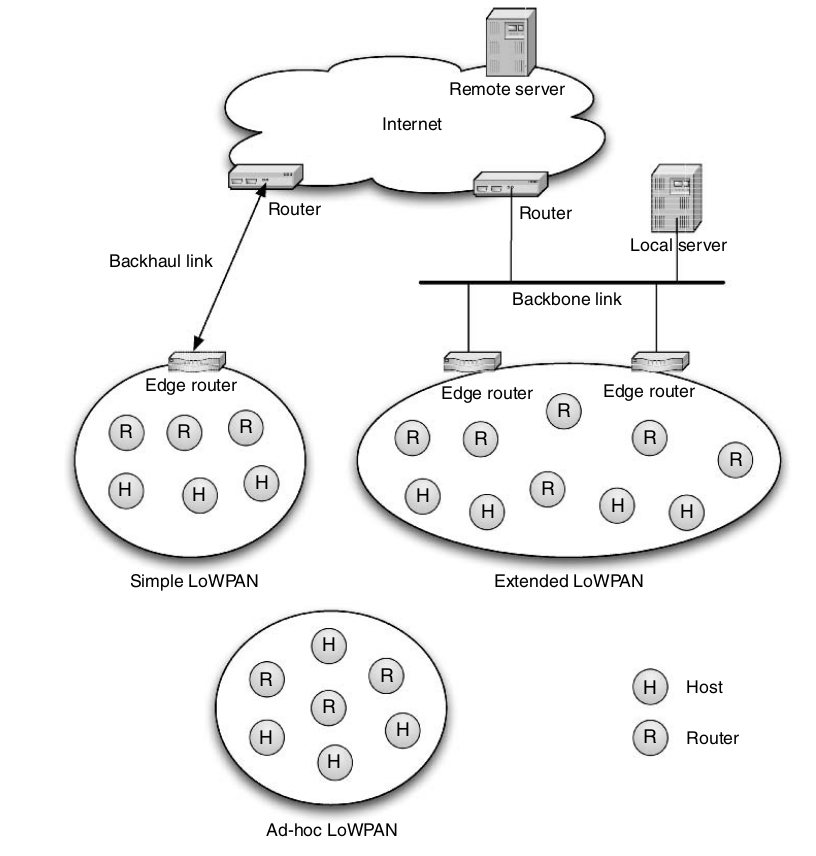
\includegraphics[width=0.8\linewidth]{lowpan}
    \caption{The 6LoWPAN architecture, see \cite[p.~14]{wie}}
    \label{fig:lowpan}
  \end{figure}

  LoWPANs are connected to other IP networks via edge routers, as illustrated in Figure 
  \ref{fig:lowpan}. The edge router plays a key role by routing traffic to and from the LoWPAN, 
  managing 6LoWPAN  compression, handling Neighbor Discovery within the network, and other network
  management features. Each node in a LoWPAN could either be a host, an edge router, or a node routing
  between other nodes. The shared common IPv6 prefix within the LoWPAN is advertised by edge routers
  or is pre-configured on each node. An edge router keeps a list of registered nodes that are accessible 
  through its network interface inside the LoWPAN.

  To enter a 6LoWPAN, a node sends a Router Solicitation message to obtain the IPv6 prefix unless it
  has been statically configured. Upon receiving the prefix, the node generates a unique global IPv6 
  address and registers this address with the edge router of the LoWPAN. This allows the edge router 
  to make informed routing decisions for traffic entering and exiting the LoWPAN, as well as to 
  facilitate neighbor discovery within the 6LoWPAN. The edge router must update the list of registered 
  nodes regularly, as addresses expire after a configurable period.  A longer expiration time 
  helps reduce a node's power consumption, while a shorter expiration time accommodates rapidly 
  changing network structures. These processes are defined in the dedicated neighbor discovery
  protocol for 6LoWPAN \cite{rfc6775}. LoWPAN nodes can travel freely within and among multiple 
  LoWPAN networks, and they may participate in several LoWPANs simultaneously. Communication 
  between a LoWPAN node and an external IP node occurs in an end-to-end manner, similar to 
  interactions between standard IP nodes.

  In an extended LoWPAN, multiple edge routers are integrated into the same LoWPAN, 
  sharing the same IPv6 prefix. These edge routers are interconnected through a common backbone link. 
  When a node moves between edge routers, it must register with the edge router it can access, 
  but it retains its IPv6 address. Communication between edge routers regarding neighbor 
  discovery is handled over the backbone link, which reduces messaging overhead. 
  This extended LoWPAN architecture allows a single LoWPAN to cover larger areas.

  An ad-hoc LoWPAN works in the same manner as a simple LoWPAN, but without the link to other
  IP networks. Instead of an edge router, a node will act as a simple edge router, handle unique 
  local address generation \cite{rfc4193} and provide the neighbor discovery registration feature 
  to other nodes.

\section{6LoWPAN Protocol Stack}
  Figure \ref{fig:ip_vs_low} depicts the IPv6 protocol stack with 6LoWPAN in comparison to a standard IP protocol 
  stack and the corresponding five layers of the Internet Model. This Internet Model 
  connects a wide range of link-layer technologies with various transport and application protocols.

  \begin{figure}[h]
    \centering
    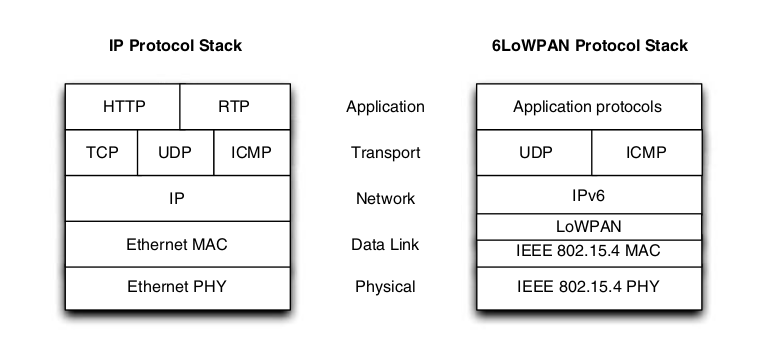
\includegraphics[width=0.8\linewidth]{ip_vs_low.png}
    \caption{IP and 6LoWPAN stack, see \cite[p.~16]{wie}}
    \label{fig:ip_vs_low}
  \end{figure}

  The IPv6 protocol stack with 6LoWPAN (sometimes called the 6LoWPAN protocol stack) is nearly 
  identical to a conventional IP stack, with a few notable differences. Primarily, 6LoWPAN only 
  supports IPv6, for which a small adaptation layer—the LoWPAN adaptation layer—has been defined 
  to optimize IPv6 for IEEE 802.15.4 and similar link layers, as detailed in \cite{rfc4944}. In practice, 
  many implementations of the 6LoWPAN stack in embedded devices combine the LoWPAN adaptation layer 
  with IPv6, allowing them to be displayed together as part of the network layer.

  The User Datagram Protocol (UDP) \cite{rfc768} is the most commonly used transport protocol 
  with 6LoWPAN, and it can be compressed using the LoWPAN format. The Transmission Control 
  Protocol (TCP) is less frequently used due to concerns about performance, efficiency, and 
  complexity, although there have been recent efforts on guidance to use and implement TCP for the IoT \cite{rfc9006}. 
  The Internet Control Message Protocol version 6 (ICMPv6) \cite{rfc4443} is utilized 
  for control messaging, including functions like ICMP echo requests, destination unreachable messages, 
  and Neighbor Discovery. While many application protocols are application-specific and in binary format, 
  there is a growing availability of more standardized application protocols.

\section{IEEE 802.15.4}
  Established by the IEEE, the IEEE 802.15.4 standards define low-power wireless radio techniques 
  and specify the physical and media access control layers that serve as the foundation for 6LoWPAN. 
  The IEEE 802.15.4-2011 version of the standards includes features such as access control via 
  CSMA/CA, optional acknowledgments for retransmission of corrupted data, and 128-bit AES encryption 
  at the link layer. It offers addressing modes that utilize both 64-bit and 16-bit addresses 
  with unicast and broadcast capabilities. The payload of a physical frame can reach up to 127 bytes, 
  with 72 to 116 bytes of the usable payload after link-layer framing, depending on different addressing 
  and security options \cite[Appendix B.1]{wie}.

  Star and point-to-point network topologies are supported by IEEE 802.15.4. The MAC layer can operate 
  with CSMA/CA in the beacon-less mode. In beacon-enabled mode, TDMA/TISCH for media access is utilized.
  The number of nodes, the length of the transmitted messages, and the level of radio interference 
  within the ISM band significantly influenced the average packet loss in IEEE 802.15.4 \cite{packet_loss}. 
  While the use of acknowledgments at the link layer enhances reliability, it complicates the 
  estimation of packet round-trip times.